%TODO: review results
%TODO: outline conclusions
%TODO: write introduction
%TODO: write methodology
%TODO: re-write results
%TODO: write conclusions
%TODO: review extensively
\documentclass[letterpaper]{sig-alternate}

\usepackage{hyperref}

\pdfpagewidth = 8.5in
\pdfpageheight = 11in

%\usepackage[factor=250,spacing=true]{microtype}

\begin{document}
\conferenceinfo{RecSys '14}{October 6--10, 2014, Foster City, Silicon Valley, USA}
%\CopyrightYear{2007} % Allows default copyright year (20XX) to be over-ridden - IF NEED BE.
%\crdata{0-12345-67-8/90/01}  % Allows default copyright data (0-89791-88-6/97/05) to be over-ridden - IF NEED BE.

\title{TODO: title}

\numberofauthors{2}

\author {
\alignauthor
Daniel Kluver\\
\affaddr{GroupLens Research}\\
\affaddr{Department of Computer Science and Engineering}\\
\affaddr{University of Minnesota}\\
\affaddr{Minneapolis, MN 55455 USA}\\
\email{kluver@cs.umn.edu}
\alignauthor
Joseph A. Konstan\\
\affaddr{GroupLens Research}\\
\affaddr{Department of Computer Science and Engineering}\\
\affaddr{University of Minnesota}\\
\affaddr{Minneapolis, MN 55455 USA}\\
\email{konstan@cs.umn.edu}
}

\maketitle
\begin{abstract}

TODO: abstract

\end{abstract}

%TODO: update these things.
% A category with the (minimum) three required fields
\category{H.4}{Information Systems Applications}{Miscellaneous}
%A category including the fourth, optional field follows...
\category{D.2.8}{Software Engineering}{Metrics}[complexity measures, performance measures]

%TODO: update these things.
\terms{Theory}

%TODO: update these things.
\keywords{ACM proceedings, \LaTeX, text tagging}

\section{Introduction}

  % new user experiance is only chance to make all important first impression
  One of the important problems in recommender systems is the new user experience.
  If the system cannot provide a good user experience, then new users are likely to leave and not return.
  Even if the user does choose to enter the system, the user's first impression of the system can have a lasting impact on how the user interacts with the system.
  The user's first impression can shape how the user expects the system to behave in future interactions, fundamentally changing how the user perceives the system.

% one important trait is trust.
    % trust is complex
    % matching user's experiance is probably important.
  %One important part of how the user interacts with a recommender system is how much the user trusts the recommender system.
  %The more the user trusts a recommender system, the more the user can take advantage of it.
  %If the user doesn't trust a recommender system, the system can be of no value to the user.
  %Building trust with the user is therefore an important part of the new user experience.
  %Past work has shown that one of the strongest factors in the formation of trust is how much the system's recommendations match the user's knowledge \cite{wangAttributionOfTrust}.
  %For new users this can easily take the form of recommending items that the user has already seen.
  %TODO: I kinda of want to cut this. I want to talk about this theme, but I don't actually know where it fits in.

  % past work tends to focus on the algorithm side, the algorithm side of this problem is cold start.
    % SMAL DATA TENDS TO IMPLY BAD RESULTS.
    % cold start algorithms is a larger problem
    % cold start algorithms tend to use extra information to help imrpove eary performance.
    % we only look at user cold start as it is ubiquitous.
  Past work on new user experience in recommender systems has tended to focus on the `cold start problem'.
  Cold start refers to the problem that no algorithm can make useful recommendations with very limited amounts of information, therefore new users and items must have worse recommendations.
  We will only discuss the user side of the cold start problem in this work.
  Most solutions to the cold start problem require some source of extra information about new users.
  
  % One common new user strategy is to have a special data collection mode.
  % collect ratings fast to get over a precived ``bad period''
  % work on this focuses on how to collect useful ratings.
  % (framework from decision tree work)
  The best studied strategy for new users is to have users go through a new user rating survey.
  Systems that take this practice do not allow their users to receive recommendations until some fixed number of ratings have been entered.
  The idea is that after enough ratings have been entered, the predictions will be `good enough'.
  This idea has been explored by many authors, most consider a system in which the user is presented with a list of items, and asked to rate items until they have enough ratings.
  For a good discussion of prior work in this direction see \cite{adaptiveBootstrapping}.
  Generally, this work strives to strike a balance between the effort user needed to get enough ratings, and the usefulness of each rating to the system.
  This balance is complicated by how effort effects the user's perception of value \cite{TenIsEnough}.

  % One promising approach is to let user control interaction
  % user or system driven control.
  % promising, we don't know much about follow up.
  One promising approach to the new user rating survey is to have users control which movies they rate.
  This was pioneered by McNee et al., who looked at comparisons between user driven and system driven new user surveys \cite{mcneeInterfaces}.
  They found that users who were in control of the items they rated made fewer ratings, but that the profiles they created were more useful in predicting the user's future ratings.
  Interestingly, while these users took more time to create their profiles, they were just as likely as other users to report that the sign up was short.
  While these results are quite promising, to our knowledge no follow up work has been done to explore these issues further.
  This goes to show, however, that the new user experience is a complicated issue and novel strategies may yet prove to be the best solution.

  % bridge from past work to our work.
    % point out holes (evaluating standard algorithms for little to no ratings, wholeistic evaluation)
    % point out that other approaches than smart object ordering exist, and we need to be able to compare.

  While past work has covered the new user rating survey as a solution to new user cold start, much less work has been done comparing other strategies.
  Most of this work has been focused on strategies for how to get ratings from users.
  Very little work has carefully considered how best to use the information we receive.
  Most authors simply assert that more ratings are better, but for new users we may see interesting performance gains by simply choosing algorithms that perform well for new users.

  We propose to combine two traditions of recommender system research, offline algorithm analysis and new user experience research.
  We seek to compare algorithms based on their performance for new users.
  Our goal is to understand the differences between algorithms for new users, especially how these algorithms respond to different amounts of information.
  While there has been much work comparing algorithms in an offline setting, very little of it has explored what are the best algorithms for users with very few ratings.
  %Furthermore, we do not seek to find the algorithm that scores best on some metric of choice, instead, we seek to form a complete understanding of the differences between algorithms for cold start use.


  We structure our work around the following research question.
  \begin{itemize}
    \item RQ1: How do algorithms behave for users with few ratings?
  \end{itemize}
  Unfortunately, algorithm behavior is a broad and hard to define subject.
  We will look at three distinct sub questions to help capture recommender system behavior.
  Each sub question may represent several actual metrics in our evaluation.
  %We will look at three distinct ways to quantify the behavior of a recommender system. each of which will lead to multiple metrics.

% RQs
    % RQ1 How do the behavior of different algorithms change with the number of ratings?
      % Explain that there are a lot of different ways to measure algorithm behavior.
        % Predictive accuracy, commonly measured with MAE or RMSE
          % coverage
        % Value of recommendations, tradidionally done with metrics from information retrieval such as precision, recall, MAP, etc. These algorithms try to measure ...
          % cite the John/Joe paper (RMSE is not enough)
          % cite the paper cited by 10 is enough
          % topN RMSE
        % There are many properties of recommenders that are (find words here)
          % popularity
          % diversity
          % spread
      
  \begin{itemize}
  \item RQ1.a: How do algorithms behave with respect to prediction accuracy?
  \item RQ1.b: How do algorithms behave with respect to ranking and recommending?
  \item RQ1.c: How do algorithms behave as measured by other metrics such as popularity and diversity?
  \end{itemize}

  We will answer these questions by developing an evaluation framework that can be used to understand how algorithms perform for new users.
  This framework will compare algorithms on eleven different metrics to allow a more complete understanding of the differences between algorithms.
  We will then use this framework to study how three common algorithms behave for new users.
  Finally, we will draw conclusions from our evaluation and outline directions for future work.

\section{Methodology}
\label{sec:methodology}
  % (high level description/restatement of approach) To answer our research questions we will various metrics of recommenders in an offline setting simulations users as they join the system.
    % maybe hit some limitations
    % motiviate _why do a simulation_ (a lot of metrics we want to try)

  To answer our research questions we will evaluate algorithms in an offline simulation designed to simulate users as they join the system.
  We will do this by running separate instances of the standard train and test methodology, each one designed so that every test user has a specific  number of ratings.
  We will then plot metric results against the number of retained items to understand both how the algorithms compare on these metrics, and how the algorithm performance changes with the number of ratings provided.
  This, or a similar technique, has been used by previous authors to make plots of metrics over profile size \cite{DrennerInitialExperiance, TenIsEnough, AdaptiveBootstrap}.
  These authors did this simply to establish that recommender accuracy does improve as the number of ratings grows.
  Therefore these authors did not carefully compare multiple algorithms on a breadth of metrics.
  We will use this technique to develop a much more nuanced understanding of the differences between algorithms.

  Our approach is related to a temporal evaluation, in which a recommender is trained on all ratings up to a point in time, and then tested using the next ratings to be made.
  Temporal evaluations have been used in the past to evaluate how the list of recommendations from different algorithms change as users enter more ratings into the system \cite{LathiaTemporal}.
  While the output of a temporal evaluation are very similar to our own, the methodology has some key differences.
  Where a temporal evaluation is designed specifically to consider the order in which users make ratings, our methodology is designed to try to eliminate this ordering effect from our consideration of the algorithm's behavior.

  As mentioned earlier, many recommender systems use a new user survey to collect the first user ratings.
  These ratings are intentionally different than normal user ratings.
  As we will discuss shortly, our methodology uses randomization in key places to remove this ordering effect.
  This allows us to better capture the underlying algorithm performance on ``normal'' user data.
  While this makes our methodology unsuited for temporal metrics, it allows us to separate an algorithm's behavior from how ratings are collected for new users.
  Therefore, we feel that our methodology is more suitable to answer our research question.

  \subsection*{Algorithms}
  % algorithms (discuss tuning of algorithms per algorithm?)
  % motivation for algorithm selection
  % list algorithms 

  We seek to develop an understanding of how a range of different standard algorithms perform at for new users.
  Rather than picking advanced algorithms that are tuned for new user performance, we decided to first understand how representatives of three common types of algorithms perform.
  Therefore we will compare User-User, Item-Item, and Simon Funk's SVD algorithms against two simple baseline algorithms.
  More information about these algorithms can be found in table \ref{tbl:algo}
  Code for our evaluation, using the Lenskit evaluation framework \cite{lenskit} is available at \url{https://bitbucket.org/kluver/coldstartrecommendation}.
  
  \begin{table}
    \centering
    \begin{tabular}{|p{6em}|p{18em}|}
      \hline
      Algorithm          & Algorithm description \\\hline
      ItemBaseline       & Item's average rating, with mild bayesian damping towards the global mean \cite{funk_netflix_2006}. \\\hline
      UserItem\-Baseline & ItemBasline adjusted by the user's average offset from the ItemBaseline. Mild mean damping is applied \cite{funk_netflix_2006}. \\\hline
      User-User          & User based nearest neighbor collaborative filtering \cite{resnick1994grouplens} with a neighborhood size of 30 and ratings normalized by subtracting the UserItemBaseline score. \\\hline
      Item-Item          & Item based nearest neighbor collaborative filtering \cite{sarwar2001item} with a neighborhood size of 30 and ratings normalized by subtracting the ItemBaseline score.   \\\hline
      SVD                & Simon Funk's SVD based collaborative filtering approach \cite{funk_netflix_2006} with 30 features and 150 training iterations per feature. \\\hline
    \end{tabular}
    \caption{Summary of algorithms.}
    \label{tbl:algo}
  \end{table}
  
  % evaluation and code to run these algortihms available at.
  % citations and lenskit info
  Each algorithm was configured and tuned similarly to Ekstrand's 2012 evaluation \cite{ekstrand2012recommenders}.
  Since this evaluation was on a different dataset (MovieLens 10M vs. MovieLens 1M), we performed minor tuning from these parameters.
  Most notable, we found that the previous damping parameter used for the baselines was too large.
  We found that a value of 5 gave much better results for new user recommendation.
  During tuning we found that our key results are consistent among those configurations that perform well.
  %TODO: carefully run this wording by joe.

  \subsection*{Metrics}
  We will discuss a total of eleven metrics.
  Some of these metrics will prove to be redundant, and future work should be able to use a much smaller list of metrics.
  The metrics are listed in table \ref{tbl:metrics}.
  \begin{table}[ht!]
    \centering
    \begin{tabular}{|p{7em}|p{16em}|}
      \hline
      \multicolumn{2}{|c|}{{\bf Accuracy Metrics}} \\\hline
      RMSE                   & Standard prediction accuracy metric. \\\hline
      \hline
      \multicolumn{2}{|c|}{{\bf Recommendation Metrics}} \\\hline
      nDCG                   & Standard ranking quality evaluation.\\\hline
      Precision@20           & Count of recommended items in the test set and rated 4.0 or higher.\\\hline
      MAP@20                 & Average of precision at each rank one through twenty.\\\hline
      Fallout@20             & Count of recommended items in the test set and rated 2.0 or lower.\\\hline
      SeenItems@20           & Count of recommended items in the test set.\\\hline
      MeanRating@20          & Average rating of recommended items that are in the test set.\\\hline
      RMSE@20                & RMSE computed only over those items that were recommended.\\\hline
      \hline
      \multicolumn{2}{|c|}{{\bf Other Metrics}} \\\hline
      Average\-Popularity@20 & The average number of users in the training set that have seen recommended items.\\\hline
      AILS@20                & The average pairwise similarity between recommended items. \\\hline
      Spread@20              & The Shannon's entropy of the distribution of recommended items for users in the test set.\\\hline
    \end{tabular}
    \caption{TODO:}
    \label{tbl:metrics}
  \end{table}
  
  All metrics evaluating recommendations (all but RMSE and nDCG) are based on the top 20 highest predicted items for the user, excluding items in the training set.
  The choice of 20 items for the evaluations was arbitrary, testing with other values showed similar results, except on one metric.
  This issue will be addressed later in the results section.
  
  Most of our metrics are standard techniques, so we will only address the latter 6.
  As we will discuss later, we found Precision, MAP, and fallout to not be useful for this evaluation, therefore to help understand the quality of our recommendations, we include SeenItems@20, MeanRating@20, and RMSE@20.
  SeemItems@20 tells us how frequently the user is to have previously seen a recommended item.
  This is useful for two reasons.
  First this provides important context for the next two metrics, as this is how many items those metrics are often averaged over.
  Secondly, if too many items are known to the user, the user might feel that the recommendations are not interesting.
  Alternatively, if too few of the items are known to the user, the user may have trouble evaluating the recommendations, which could lead the user to leave the system.

  MeanRatings@20, and RMSE@20 both try to establish how much the user likes the recommendations.
  MeanRatings@20 tells us directly how much the user tends to like recommended movies.
  RMSE@20 accompanies this and lets us know if the recommended items are likely to be mispredicted, which can explain why users may or may not like their recommendations.

  The average popularity metric is a crude metric of how novel the recommendations are to the user \cite{zieglerDiversity}.
  Broadly speaking we expect users will prefer recommendation lists containing more novel (less popular) items.
  However, if the recommended items are too unpopular we risk that the user will not have heard of the items, which could make the user doubt the recommendations, hurting the user experiance.

  Past work has shown that users like their recommendations to be more diverse \cite{zieglerDiversity, martijnDiversity}.
  The belief is that by providing more diverse lists we are giving the user a larger range of items to choose from.
  This can make choosing an item easier as the user is less likely to have to compare very similar options.
  We will measure diversity with the AILS@20 metric.

  The AILS@20 metric is based on the ILS metric introduced by ziegler et al \cite{zieglerDiversity}.
  AILS@N is simply a rescaling of ILS to be scale free with regards to N, this was done to make the metric easier to interpret, by putting it on the same scale as similarity values.
  We used the same item similarity metric for AILS@20 as we used in the Item-Item recommender.

  The Spread@20 metric is designed to measure how well the recommender spreads its attention across many items.
  We expect that algorithms with a good understanding of its users will be able to recommend different items to different users.
  Spread is computed by computing recommendations for each test user.
  Let $C(I)$ be the count of how many times item $I$ showed up in the recommendations.
  Let $P(I) = C(I) / \sum_I C(I)$ be the probability that a random recommendation is item $I$.
  Finally we define spread as the Shannon's entropy of $P(I)$, $Spread = -\sum_I P(I) \log(P(I))$.
  When this is large we know that the recommender is recommending many items with a relatively even distribution.
  When this is low, the recommender is focusing on a small set of items which it recommends to every user.

  % provide expectations.
  We expect that the item baseline algorithm will have approximately constant performance on all metrics.
  Since the Item Baseline is such a simple algorithm we expect that any reasonable algorithm should be able to do better on it on the accuracy and recommendation metrics.
  Furthermore, we expect the improvement over the item baseline to be gradual, with larger improvements only happening with more data.

  The user-item baseline should only differ from the item baseline for metrics that use the prediction value.
  For all other metrics these two should provide the same responses.
  As the user-item baseline is still quite a simple baseline, we expect that each algorithm will beat this baseline as well.
  That said, for small rating values its possible that the improvements over this baseline will be very minimal.
  
  We expect that the baseline algorithms will provide the most popular recommendations, with the least diversity, and the least spread.
  We expect that any personalized algorithm should be able to make more nuanced recommendations than simply recommending the best rated items, which should translate as gains on these metrics.  
  
  \subsection*{Dataset}
  % dataset
    % # user
    % # items
    % distributions of # ratings per user (important: min 20)
    % establish range of evaluation.
  For this evaluation we will use the MovieLens 1M dataset.

  % movielens system
      % silly cold start
      % randomization
  The MovieLens system uses a new user rating survey to allow users to enter the system.
  
  \subsection*{Evaluation Procedure}
  % subsampling strategy
  % describe normal crossfold solution
  The natural way to perform this evaluation is with a modified user crossfolding strategy.
  
  % describe issues with solution
  Unfortunately, we found that this strategy can causes biases in our evaluation.
  
  % describe our crossfold then subsample solution.
  Our solution to this bais is to subsample an existing crossfold.

\section{Results}

  Using the methodology described in section \ref{sec:methodology} we generate plots for each metric showing how the five algorithms perform new users.
  Where appropriate, we will compute metrics independently for each user, and plot the average user value, with a 95\% confidence interval around this mean.
  Where this cannot be done we will compute the metric once for each of the five folds, and plot the values for each fold, with a lines through the average.

\subsection{Prediction accuracy}
  % Prediction accuracy
\begin{figure*}
  \centering

  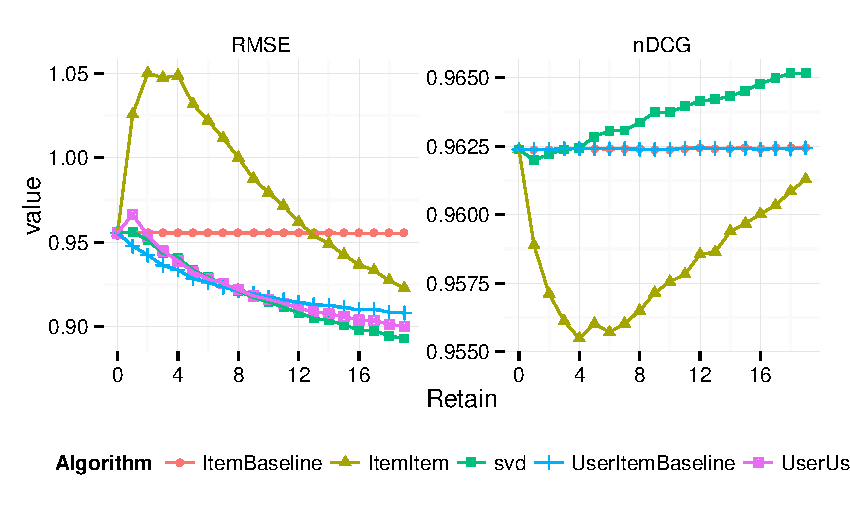
\includegraphics[width=\linewidth]{../lenskit/output/ekstrandTuned20/accuracy.pdf}
  \caption{Left: RMSE, Right: nDCG}
  \label{fig:rmse}
  \label{fig:ndcg}
\end{figure*}
    % RMSE plot
    % point out error bars etc.
    % explain / interpret plot
  Figure \ref{fig:rmse} shows how accurate our algorithms are as measured by RMSE.
  As would be expected the accuracy of our item baseline doesn't change as the amount of information changes.
  The User-User and svd algorithms both perform as expected, starting out with the same accuracy as the item baseline, and then monotonically improving.
  User-User does show a small increase of error with only one rating, but the change is quite small and unlikely to be noticed by users.
  Interestingly, User-User and svd both perform about as well as our smarter user item baseline. %TODO: explain this better

      % explain strangeness of Item-Item
  Item-Item performs quite poorly in the cold start setting.
  Until we have around 20 ratings the RMSE of Item-Item is worse than the item baseline.
  More interestingly, unlike the other algorithms Item-Item actually appears to performs worse as it gets more ratings for the first few ratings.
  
  The curve exhibited by Item-Item's RMSE is caused by two trends.
  First as the system revives more ratings, predictions from Item-Item are more accurate, leading to a downward trend.
  Secondly, as the system revives more ratings, Item-Item can make predictions for more items, meaning the fewer predictions are serviced by the baseline.
  Because the baseline is more accurate, this leads to an upward trend.
  Overall this leads to curved performance.
  If we were to compute RMSE only over the items where item-item can make a prediction we would see a curve similar to the other algorithms, but shifted up.
      % possibly coverage plot
      % true crossing point?

\subsection {Recommendatin quality metrics}
  % Recommendation quality metrics
    % NDCG
  Figure \ref{fig:ndcg} shows the algorithm's performance on the nDCG metric.
  The algorithm's behavior is essentially equivalent to the RMSE behavior.
  Again, User-User has a minor dip on very new users, but then tracks SVD in uniformly improving quite well from there.
  Likewise Item-Item exhibits the same dipped accuracy, although it doesn't catch up the baseline as fast.
  Unlike previous metrics, the item baseline, and the user-item baseline have the same performance.
  This is because nDCG is a ranking metric, not an accuracy metric.
  Because the user item baseline orders items the same way as the item baseline, both will have the same accuracy on any ranking metrics.

    % MAP, precision, fallout plots 
    % explain results from MAP and precision
    % explain recall results
    % recall results, strangeness and popularity


\begin{figure*}[ht!]
  \centering
  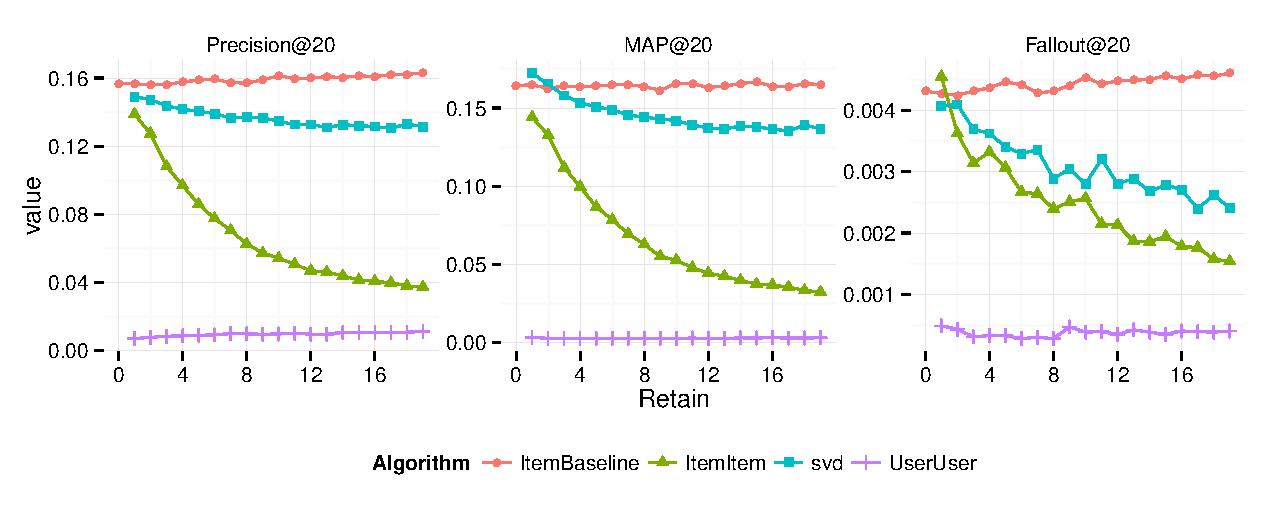
\includegraphics[width=1.1\linewidth]{../lenskit/output/ekstrandTuned20/TopNPrecision.pdf}
  \caption{TODO}
  \label{fig:map}
\end{figure*}


  Figure \ref{fig:map} shows MAP@20, precision@20, and fallout@20.
  All three metrics show essentially the same trend, User-User gets the lowest score, the baselines get the highest score.
  On both MAP@20 and precision@20 svd gets a higher score than Item-Item throughout, performing almost as highly as the baseline.
  On fallout@20 Item-Item performs higher than svd and the baseline, but decreases faster than bath, ending with a lower score than either. 
  We also tried recall@20 and mrr@20 and found the same trend.

  This result is rather strange as MAP and precision are metrics where high scores imply better performance, whereas fallout is a metric where high scores imply poor performance.
  This leads to an issue, these metrics contradict each other in terms of the quality of the recommendations from our algorithm.
  One possible reason for this is that these topN metrics are known to be biased toward recommendations that have more popular items \cite{bellogin}.
  Looking at the average popularity (figure \ref{fig:pop}) of recommended items, we see that the average popularity of the recommendations closely replicates the previous three plots.
  Therefore we seek a different, less biased metric to analyze the quality of the recommendations.


  % TopN average rating / topn rmse
    % interpret graph and reason about what it means about quality

\begin{figure*}[ht!]
  \centering
  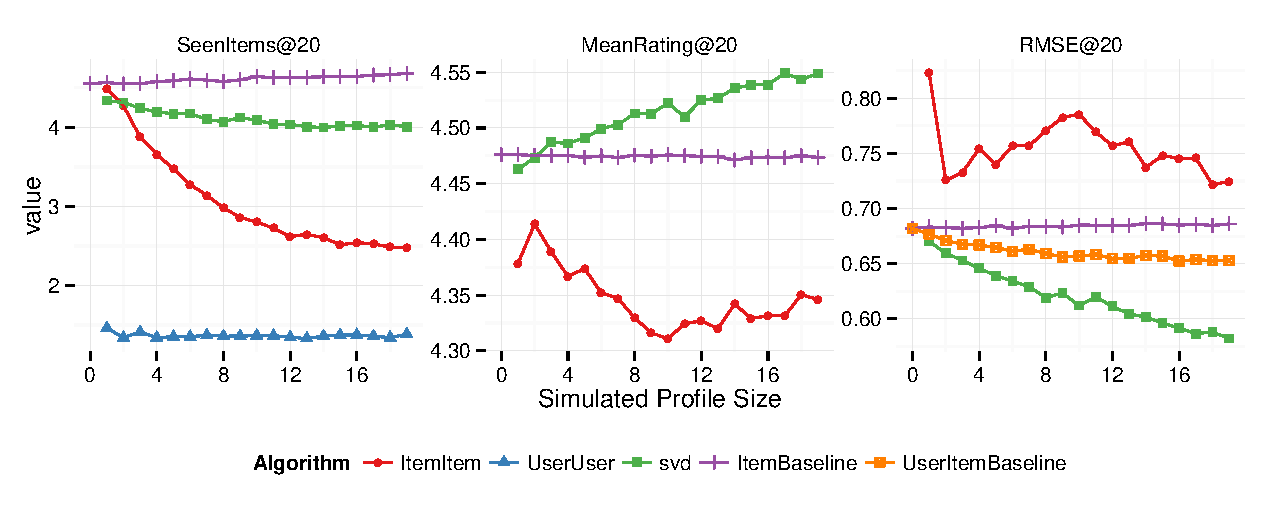
\includegraphics[width=1.1\linewidth]{../lenskit/output/ekstrandTuned20/rmse_20.pdf}
  \caption{TODO}
  \label{fig:topN.rmse}
\end{figure*}


  The first graph in figure \ref{fig:topN.rmse} shows the average number of items in the top 20 recommendations for each algorithm that were also in the test set.
  The average number of test set items in recommendations shows a similar trend to the MAP, precision, and recall metrics, user-user getting by far the fewest seen items, and the baseline getting the most.
  %TODO: talk about trust building here!

  The second graph in figure \ref{fig:topN.rmse} shows the average rating for those items in the top 20 recommendations for each algorithm.
  The first thing to note about this graph is that all of these algorithms are doing a reasonable job of recommending items the user might like to watch, with all algorithms averaging above 4 stars (implying that the recommended items are, at least on average, enjoyable).
  SVD performs as expected, starting at close to the same average rating as the baselines, and then slowing improving as more ratings are entered.
  Item-Item performs poorly, not only performing worse than the baseline, but showing worse performance as more ratings are added.
  This is quite possibly a similar trend to the one we observed with RMSE and nDCG, where Item-Item's performance decreased as coverage increased leading to the curved performance at cold start.
  
  During testing with other values of N for this metric and the next, we found that User-User's behavior compared to the other algorithms changed significantly with different values of N.
  This is probably due to the very low rate of having seen items in the recommendations, which makes its value much less stable, than the other algorithms.
  Because of this behavior we will draw no conclusion from User-User's performance on this metric, to avoid accidentally attributing behavior to it, that was instead formed by our choice of 20 as N.
  
  The third graph in figure \ref{fig:topN.rmse} shows the RMSE our algorithms got on items in the top 20 recommendations for each algorithm.
  Not surprisingly, this figure shows the same trends as the last one meaning that the algorithms whose recommendations were (on average) most likable, were those whose recommendations were most accurate.
  Again, SVD performs quite well, Item-Item shows poor performance, and, due to sensitivity of User-User to our choice of N, we make no conclusions about User-User.

\subsection{Other recommender metrics}
  % Other recommender metrics

\begin{figure*}[ht!]
  \centering
  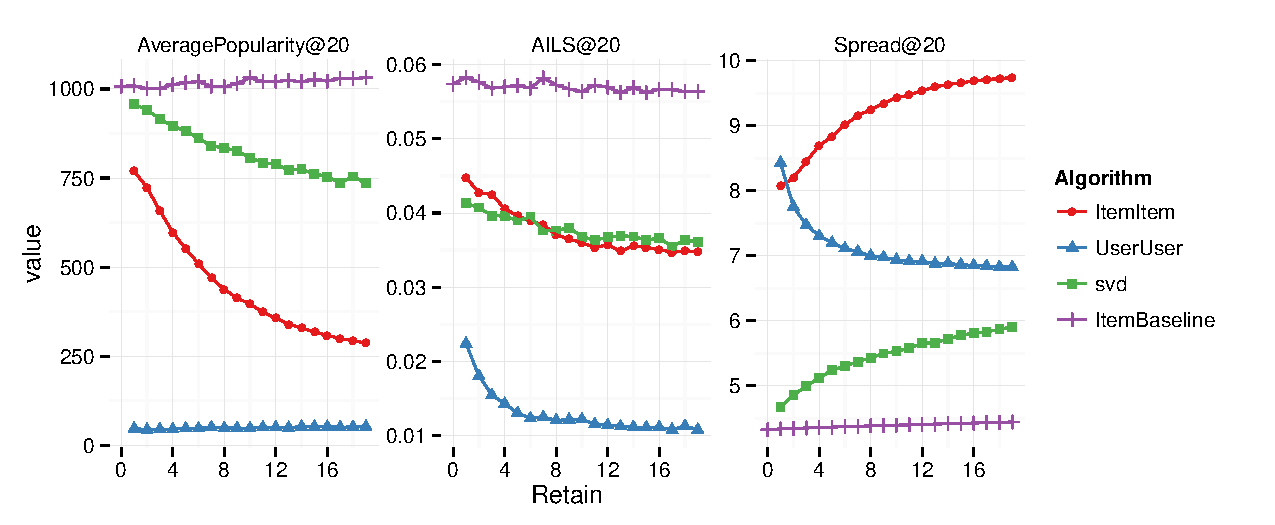
\includegraphics[width=\linewidth]{../lenskit/output/ekstrandTuned20/popdiv.pdf}
  \caption{TODO}
  \label{fig:pop}
\end{figure*}


    % popularity graph
  The first graph in figure \ref{fig:pop} shows the average popularity of recommended items by each algorithm.
  %TODO: re-write this
  Across all datapoint sizes the ranking of algorithms is the same, with the baselines recommending the most popular movies, followed by svd, which recommends less popular movies, then Item-Item, which recommends much less popular movies, leaving User-User to recommend the least popular movies.
  Unfortunately, we don't know of any guideline for understanding how popular users desire their recommendations to be.
  That in mind, we expect that users will feel the baseline's popularity (around 1000) is too high, and User-User's popularity (around 50) is too low.
  SVD and Item-Item both seem to perform well, with SVD generating more popular recommendations, than Item-Item, and both algorithms showing a significant trend to make less popular predictions as we know more about the user.

    % diversity plot
  The diversity graph in \ref{fig:pop} shows a similar trend to the popularity trend with the baseline algorithms producing the least diverse list of recommendations and User-User providing by far the most diverse list of recommendations.
  For the first few ratings SVD is able to provide more diverse recommendations than Item-Item.
  However, Item-Item seems to grow in diversity faster than SVD in response to more data, so after 4 ratings Item-Item is providing slightly more diverse recommendations than SVD.
  Overall, Item-Item and SVD are providing recommendations that, at least in an offline context, appear to have quite comparable diversity.


\begin{figure}[ht!]
  \centering
  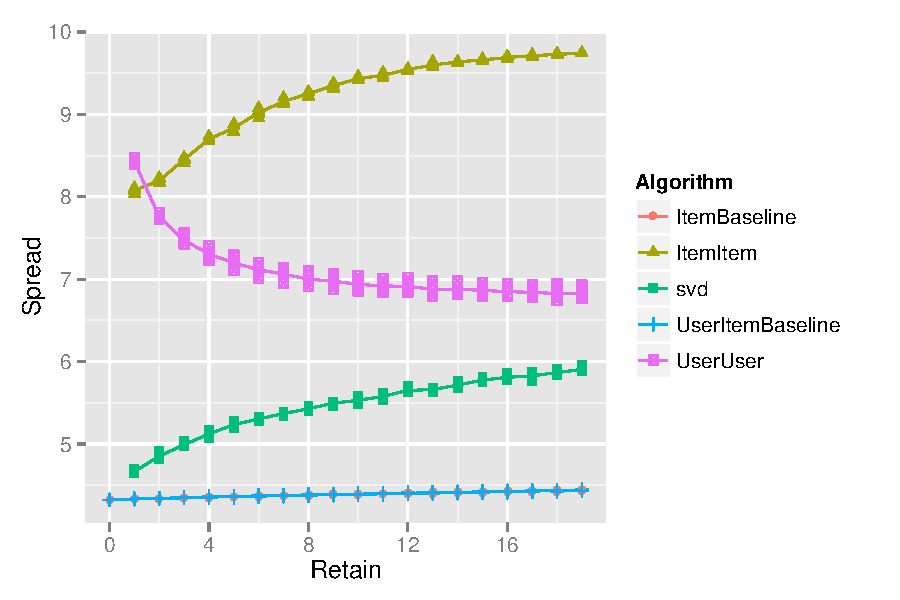
\includegraphics[width=1.1\columnwidth]{../lenskit/output/ekstrandTuned20/topN_entropy.pdf}
  \caption{TODO}
  \label{fig:spread}
\end{figure}


  % spread plot
  The graph in \ref{fig:spread} shows the spread of the recommendations from each algorithm.
  Because this metric can only be computed over a group of people, confidence intervals over the per-user average are not provided, instead the specific spread values computed in each five folds are shown as points, with lines connecting the value from the five metrics.
  %TODO: make this point earier and better.
  Like the diversity and popularity metrics we see that the values take a much larger range, with different algorithms seeming to converge to different amounts spread.
  The baseline algorithms, which recommend every user the same list of recommendations (unless the user has rated one of those items) have the lowest spread.
  SVD has the second lowest spread, starting with a spread very close to the baselines and then slowly growing more spread as it gets more ratings.
  Like popularity, we don't know exactly how much spread is best for a recommender system, but we can guess that we want more spread from our recommendations than baseline, and all other things being equal, more spread is probably better.
  Based on this intuition it seems that SVD might have focus on too few items in its recommendations.

  User-User and Item-Item both have significantly more spread than the other algorithms.
  They show interestingly opposite trends, with User-User providing more spread at one rating, and then decreasing, and Item-Item giving less spread and then increasing.
  By 8 ratings, we see that Item-Item has by far the most spread recommendations.
  It is strange that User-User would get less spread as it learns more about users.
  This implies that the more it learns about users, the less spread out its recommendations are.
  This could be some form of a regression towards the mean, where as it learns more about users its recommendations become less personalized to the users individual quirks.
  More research will be needed to understand this trend.
  
\section{Conclusions}
  % summary of results in a big old table.
    % the accuracy of svd and user-user both seemed good. item-item seemed to have trouble especially with very new users.
    % svd did quite well on our traditional topN metrics, item-item did OK, and user-user did bad., but there are flaws with these metrics.
    % on our topN RMSE item-item (again) seemed to have issues, and user-user did quite well, but the low hit rate is troubleing. 
    % again svd seems the winner here.
    % on our fluffy metrics item-item and svd seemed to do well. I might argue that item-item seemed to do better (spread, and higher throughout).
    % user-user seemed to do poor
  % what this means
    % user-user seems to be able to give accurate predictions, but seems to focus on overly obscure items in recommendation.
    % item-item seems to give not-bad recommendations, but its predictions have issues
    % based only on these results svd seems to be the best performer and is our recommendation to new systems.
  % other takeaways
    % regularization
    % if you use a switching recommender, this methodology can help you choose when to switch.
    % non-traditional metrics can tell you more about what is going on, these seem to be more properties of the class of algo than of the data, so its worth looking at these when choosing algorithms, to find one with properties that are good for your task.

  % limitations and opprotunities
    % dataset limitations
      % only one domain
      % no quitters in our dataset
    % metrics limitations
      % many metrics require user data to help us understand what users want from a recommender
      % no well known ``goodness'' metric for topN.
    % algorithm limitations
      % only covered three common families,
      % different algos tuned specifically for cold start.
      % algos that use extra data about users or about items.
    % cite the comparison work at CHI.

  % despite the limitations we were able to show differences between algorithms in a cold start situation.

\section{Acknowledgements}
 TODO:

\bibliographystyle{abbrv}
\bibliography{resources}  % sigproc.bib is the name of the Bibliography in this case

\end{document}
